\documentclass[10pt]{book}

%These tell TeX which packages to use.
\usepackage{array,epsfig}
\usepackage{amsmath}
\usepackage{amsfonts}
\usepackage{amssymb}
\usepackage{amsxtra}
\usepackage{amsthm}
\usepackage{mathrsfs}
\usepackage{color}
\usepackage{enumitem}

\usepackage{pgfplots}
\pgfplotsset{compat=1.6}

\pgfplotsset{soldot/.style={color=black,only marks,mark=*}} \pgfplotsset{holdot/.style={color=black,fill=white,only marks,mark=*}}

%Here I define some theorem styles and shortcut commands for symbols I use often
\theoremstyle{definition}
\newtheorem{defn}{Definition}
\newtheorem{thm}{Theorem}
\newtheorem{cor}{Corollary}
\newtheorem*{rmk}{Remark}
\newtheorem{lem}{Lemma}
\newtheorem*{joke}{Joke}
\newtheorem{ex}{Example}
\newtheorem*{soln}{Solution}
\newtheorem{prop}{Proposition}

\newcommand{\lra}{\longrightarrow}
\newcommand{\ra}{\rightarrow}
\newcommand{\surj}{\twoheadrightarrow}
\newcommand{\graph}{\mathrm{graph}}
\newcommand{\bb}[1]{\mathbb{#1}}
\newcommand{\Z}{\bb{Z}}
\newcommand{\Q}{\bb{Q}}
\newcommand{\R}{\bb{R}}
\newcommand{\C}{\bb{C}}
\newcommand{\N}{\bb{N}}
\newcommand{\M}{\mathbf{M}}
\newcommand{\m}{\mathbf{m}}
\newcommand{\MM}{\mathscr{M}}
\newcommand{\HH}{\mathscr{H}}
\newcommand{\Om}{\Omega}
\newcommand{\Ho}{\in\HH(\Om)}
\newcommand{\bd}{\partial}
\newcommand{\del}{\partial}
\newcommand{\bardel}{\overline\partial}
\newcommand{\textdf}[1]{\textbf{\textsf{#1}}\index{#1}}
\newcommand{\img}{\mathrm{img}}
\newcommand{\ip}[2]{\left\langle{#1},{#2}\right\rangle}
\newcommand{\inter}[1]{\mathrm{int}{#1}}
\newcommand{\exter}[1]{\mathrm{ext}{#1}}
\newcommand{\cl}[1]{\mathrm{cl}{#1}}
\newcommand{\ds}{\displaystyle}
\newcommand{\vol}{\mathrm{vol}}
\newcommand{\cnt}{\mathrm{ct}}
\newcommand{\osc}{\mathrm{osc}}
\newcommand{\LL}{\mathbf{L}}
\newcommand{\UU}{\mathbf{U}}
\newcommand{\support}{\mathrm{support}}
\newcommand{\AND}{\;\wedge\;}
\newcommand{\OR}{\;\vee\;}
\newcommand{\Oset}{\varnothing}
\newcommand{\st}{\ni}
\newcommand{\wh}{\widehat}
%Pagination stuff.
\setlength{\topmargin}{-0.75in}
\setlength{\oddsidemargin}{0in}
\setlength{\evensidemargin}{0in}
\setlength{\textheight}{9.in}
\setlength{\textwidth}{6.5in}
\pagestyle{empty}
\begin{document}
\begin{flushleft}
Name:\underline{\hspace{13cm}}Date:\underline{\hspace{2cm}}
\end{flushleft}
\begin{center}
{\Large Math 1041-012 \hspace{0.5cm} Quiz \#2}
\end{center}
\vspace{0.2 cm}
\subsection*{Problem 1} The graphs of $f(x)$ and $g(x)$ are given below. Use them to evaluate each limit, if it exists. If a limit does not exist explain why?
\begin{figure}[h]
    \centering
    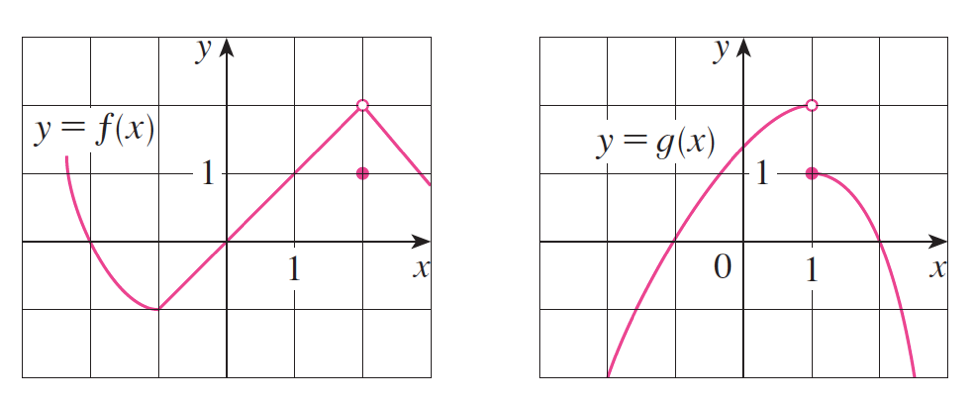
\includegraphics[width=4in]{fandg.png}
\end{figure}
\begin{enumerate}[label=(\alph*)]
    \item $\displaystyle \lim_{x\rightarrow 2}\left(4f(x)-g(x)\right)$ \vspace{1.5cm}
    \item $\displaystyle \lim_{x\rightarrow 2}\left(f(x)g(x)\right)$\vspace{1.5cm}
    \item $\displaystyle \lim_{x\rightarrow -1}\left(f(x)g(x)+x^2+1\right)$\vspace{1.5cm}
    \item $\displaystyle \lim_{x\rightarrow 0}\frac{g(x)}{f(x)}$\vspace{1.5cm}
    \item $\displaystyle \lim_{x\rightarrow 1^-}\left(f(x)+g(x)\right)$
\end{enumerate}
\raggedbottom
\pagebreak
\subsection*{Problem 2} Evaluate the limit, if it exists. Show work for partial credit.
\begin{enumerate}[label=(\alph*)]
    \item $\displaystyle \lim_{x\rightarrow 5}\frac{x^2-6x+5}{x-5}$\vspace{3.75cm}
    \item $\displaystyle \lim_{h\rightarrow 0}\frac{(-5+h)^2-25}{h}$\vspace{3.75cm}
    \item $\displaystyle \lim_{x\rightarrow 2}\frac{\sqrt{5x+6}-4}{x-2}$\vspace{3.75cm}
    \item $\displaystyle \lim_{x\rightarrow 0}\frac{|x|}{2x}$\vspace{3.75cm}
    \item $\displaystyle \lim_{x\rightarrow 3^+}\frac{1-4x}{x-3}$
\end{enumerate}
\end{document}